\documentclass{article}

% Language setting
% Replace `english' with e.g. `spanish' to change the document language
\usepackage[french]{babel}
\usepackage[fleqn]{amsmath} % Aligner les équations à gauche


% Set page size and margins
% Replace `letterpaper' with`a4paper' for UK/EU standard size
\usepackage[letterpaper,top=2cm,bottom=2cm,left=3cm,right=3cm,marginparwidth=1.75cm]{geometry}

% Useful packages

\usepackage{amsmath}
\usepackage{graphicx}
\usepackage{subcaption}
\usepackage[colorlinks=true, allcolors=blue]{hyperref}

\title{TD - Interférences }
\author{IPESUP - MP }
\date{20/09/2024}

\begin{document}
\maketitle



\section{Rappels de cours}

Pour des interférences au point $M$ entre des ondes issues de deux sources \textbf{ponctuelles, de même pulsation et synchrones} notées $S_1$ et $S_2$, on a : \\
\begin{enumerate}
  \item Différence de marche: $\delta = (S_2M) - (S_1M)$
  \item Ordre d'interférence: $p=\frac{\Delta \varphi }{2 \pi} = \frac{\delta}{\lambda}$. 
  \item Formule de Fresnel: $I(M) = I_1(M) + I_2(M) + 2 cos (\Delta \varphi) \sqrt{I_1(M) I_2(M) } $
\end{enumerate}

\textbf{Anecdote: } Grâce à son expérience des trous éponymes, Thomas Young a pu démontrer la nature ondulatoire de la lumière en 1801. 
Jusqu'alors, l'approche corpusculaire, défendue par Newton, était largement acceptée par la communauté scientifique. 
Face à l'argument d'autorité que représentait Newton, Young a eu du mal à faire entendre sa théorie. 

\section{Exercices sur les trous d'Young}

\begin{enumerate}
  \item On considère le dispositif des trous d'Young dans l'air, éclairé en incidence normale par une onde monochromatique ($\lambda =600 nm$).  on obtient une interfrange $i_0 = 2,0mm$.  On immerge le dispositif dans l'eau d'indice optique $n_1 = 1,33$.   Quelle est la nouvelle valeur de l'interfrange ? 
  \item On sort le dispositif de l'eau et on place devant un des trous un tube de longueur $L=20,0cm$ contenant du vide. On remplit lentement le tube d'air et on voit 99 franges défiler au centre de l'écran. En déduire la valeur de l'indice de l'air.  
\end{enumerate}

\section{Interféromètre stellaire}
On considère une dispositif de trous d'Young écartés d'une longueur $a$ orienté vers une étoile double de direction angulaire $+ \frac{\alpha}{2}$ et $- \frac{ \alpha}{2}$. 
Derrière le dispositif de trous d'Young, on place une lentille convergente de distance focale image $f'$. 
On place un écran dans le plan focal image de la lentille. 
On place un filtre monochromatique qui ne laisse passer que la longueur d'onde $\lambda_0 = 600nm.$
On observe que la plus petite valeur de $a$ pour laquelle on obtient un brouillage des franges est $a=1,2m$. 
En déduire la valeur de $\alpha$. 



\begin{figure}[h!]
  \centering
  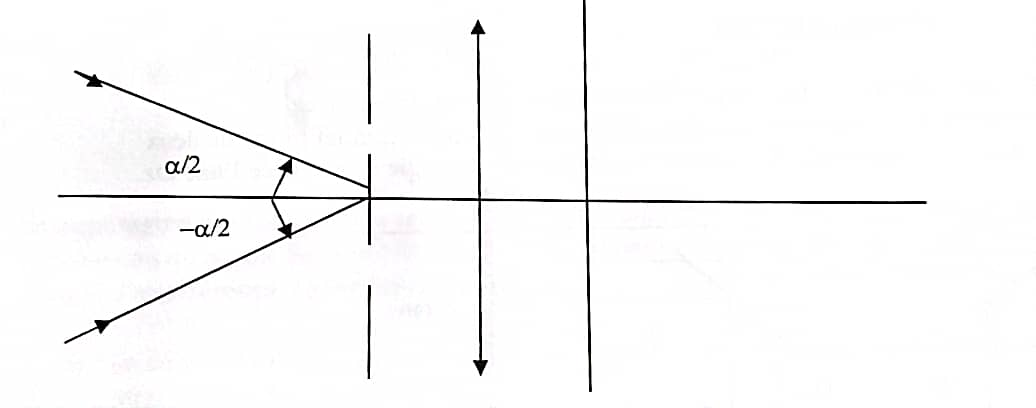
\includegraphics[width=0.4\textwidth]{interféromètre stellaire .jpg}
  \label{fig:maison}
    \caption{Schéma du dispositif}
\end{figure}

\section{Vélocimétrie laser}

On considère deux ondes planes, synchrones et de même longueur d'onde $\lambda = 514 nm$ se propageant dans des directions décalées d'un angle $2 \alpha$. 
\begin{enumerate}
  \item Faire un schéma et décrire un dispositif expérimental permettant d'obtenir une telle situation. 
  \item Dans le champ d'interférences, on fait passer des particules de vitesse $v$ et de rayon $a$ qui diffusent la lumière. Une photodiode reçoit un signal de fréquence $f=2,34MHz$. Déterminer la vitesse des particules. 
  \item On observe que le signal enregistré a une largeur $\delta f$. Expliquer son origine et en donner un ordre de grandeur en fonction des données du problème. 
\end{enumerate} 

\section{Compléments sur les trous d'Young}

Analyser l'impact d'une source étendue et d'une source non monochromatique sur l'observation d'interférences avec le dispositif des trous d'Young. 
Déterminer la période spatiale de brouillage. \\[3cm]


\begin{figure}[h]
  \centering
  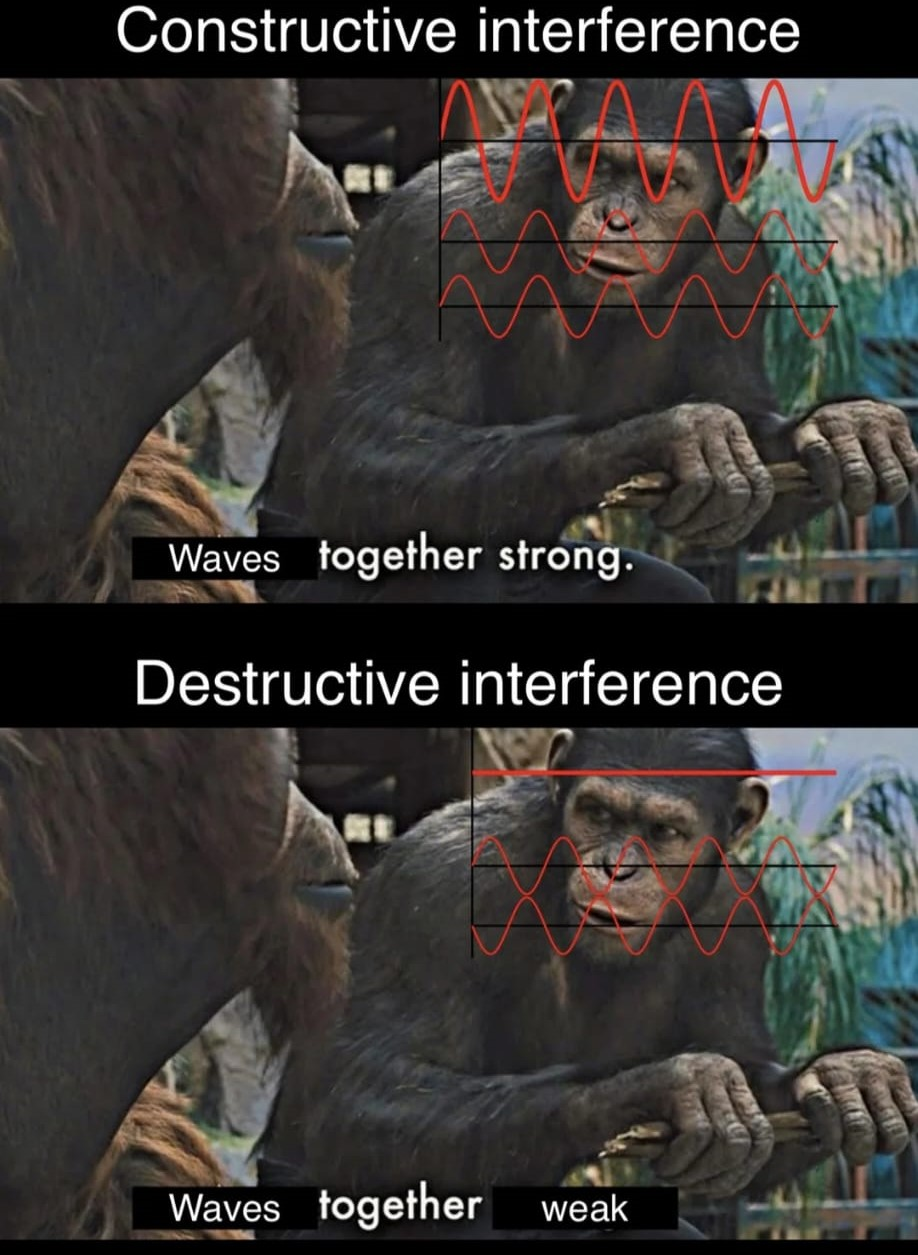
\includegraphics[width=0.4\textwidth]{meme_singes.jpg}
\end{figure}
\end{document}
*

\section*{Raéppzls de cours}

Pour des interférences au point $M$ entre des ondes issues de deux sources \textbf{ponctuelles, de même pulsation et synchrones} notées $S_1$ et $S_2$, on a : \\
\begin{enumerate}
  \item Différence de marche: $\delta = (S_2M) - (S_1M)$
  \item Ordre d'interférence: $p=\frac{\Delta \varphi }{2 \pi}$. 
  \item Formule de Fresnel: $I(M) = I_1(M) + I_2(M) + 2 \sqrt{I_1(M) I_2(M) cos (\Delta \varphi)}$
  \item Anecdote: Grâce à son expérience des trous éponymes, Thomas Young a pu démontrer la nature ondulatoire de la lumière en 1801.

